%% ==============================================
%%                   Evaluation
%% ==============================================
%% Author: Fabian Sorn
%% ==============================================

\chapter{Evaluation}
\label{ch:Evaluation}

This chapter will focus on the evaluation of the framework. The biggest question
when it comes to evaluating performance of widgetmark is, how much overhead it
is adding compared to a standard application. To evaluate the accuracy of our
benchmarking framework, we will compare the times measured in a simple example
use case with an actual implementation as a PyQt application. To
measure the timing in the application implementation, we will record timestamps
from which we can calculate the average frame rate afterwards. The use case we
will implement will be a simple use cases using PyQtGraph to plot a single curve
with 1000, 10,000, 50,000 and 100,000 points in it. 

Both variants were executed on the same hardware with the same screen
resolution as well as the same window size. Table \ref{tab:evaluation} compares
the measured frame rates for each use case.

\begin{table}[h]
\begin{center}

\captionof{table}{
    Frame rate comparison between widgetmark and a pure PyQt application
}
\label{tab:evaluation}

\begin{tabular}{rrr}

\hline
Dataset Size & Widgetmark & PyQt Application \\
\hline
1000         & 58.8       & 59.8             \\
10000        & 59.7       & 59.6             \\
500000       & 23.8       & 25.9             \\
1000000      & 12.5       & 13.9             \\
\hline

\end{tabular}
\end{center}
\end{table}

Figure \ref{fig:evaluation} compares the average recorded $\Delta t$ as well as
the standard deviation of the records. In section \ref{sec:appendix:evaluation}
are these values visually compared in more detail.

It can be seen that framework does indeed add a measurable overhead to the
execution of the use case.

\begin{figure}[h]
    \centering
    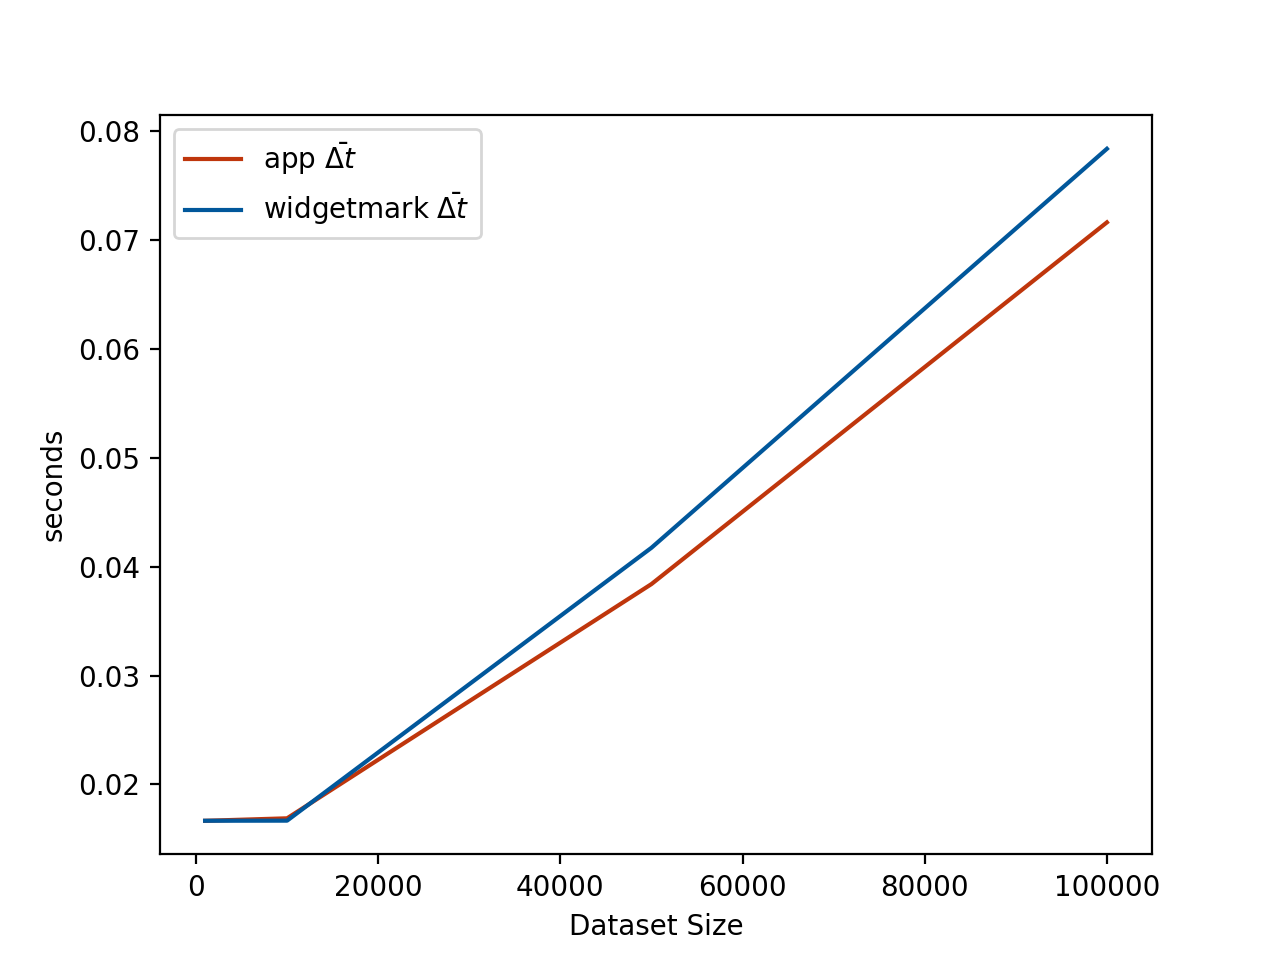
\includegraphics[width=15cm]{resources/img/evaluation/Eval_AVG}
    \caption{
        Average Delta Time and standard deviation depending on the data set
        size
    }
    \label{fig:evaluation}
\end{figure}
